%
%
%/******************************************************************************
% *filename:		shejisilu.tex
% *author:  		synckey
% *version: 		v1.0
% *datetime:		2011-06-24 14:21:17
% *description:
% *****************************************************************************/
\section{设计思路、折衷以及性能提升} 
\subsection{TCP OR UDP?}
由于可以在一个请求中接受多个域名的查询,所以数据包可能会非常大。UDP缺乏流控制和
错误控制,在数据量比较小的时候使用UDP非常合适。我们一个请求和应答的数据包可
能达到几十K,考虑到客户端的网络流量,如果使用UDP,肯定会发生错误或丢包,在应用程
序中处理错误和重传会造成资源浪费,加重服务器的负担,也会造成网络的拥堵,同时也加
大了客户的响应时间。
\par{而在数据量比较小的时候,使用UDP就非常合适。所以我们初步设计为提供两个服务器
,一个UDP服务器,和一个TCP服务器。客户端根据它的报文大小来选择使用UDP还是TCP。}
\subsection{为什么是LIRS而不是LRU?}
根据资料显示\cite{LIRS},LIRS的效率比LRU高,但是实现的代价比LRU高不了多少,所以使用LIRS。
\par{LIRS算法同时考虑到访问时间和访问频率,采用分级思想:第一级是HIR,第二级是
LIR,数据先进入到第一级,当数据在较短的时间内被访问两次时成为热点数据则进入LIR,
HIR和LIR内部都采用LRU策略。这样,LIRS中的数据比较稳定,解决了循环扫描未命中和循
环访问数据集大于缓存大小而未命中的情况,进而提高了缓存访问命中率,提高系统性能。
}
\subsection{为什么是字典树,而不使用HASH函数?} 
采用字典树与HASH函数相比,有以下几点优势:
\begin{asparaenum}[1.]
\item{可以利用字符串的公共前缀来节约存储空间} 
\item{查找效率比HASH高\cite{DATA}}
\item{不会产生碰撞} 
\end{asparaenum}

\subsection{为什么使用两个双数组字典树?}
字典树的查询效率非常高,但是动态构造的过程非常慢,需要做大量的内存拷贝。在设计中使用
两个双数组字典树。把访问频度最高的几百万(可配置的数目)个域名存放在文件中,在系
统启动时,从文件中读入域名信息,用于构造主字典树(在已知大小时,字典树构造速度非常
快,因为不需要内存的动态分配和拷贝操作)。在查询域名时,首先从主字典树中查询,如
果未命中,就把相应域名加入副字典树中(副字典树比较小,动态构造小的字典树代价很低)。
这种方式,既保留了字典树的较高的查询速率,又避免了动态构造很大的字典树带来的开销
。

\subsection{两次返回报文提升性能}
采用“一次查询两次返回”机制,对用户发送的请求报文进行两次结果返回。首先将DNS缓存
中命中的用户解析请求结果进行一次结果返回,然后将未命中的用户解析请求通过向DNS服务
器发送请求,将DNS服务器的请求结果进行二次结果返回。从而减少系统响应时间,提高系统性能。
\begin{figure}[H]                                                                                                                                       
\centering
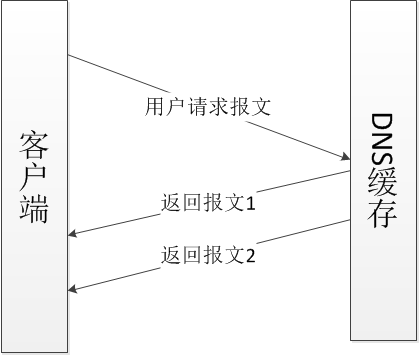
\includegraphics[keepaspectratio, scale=0.8]{pitures/one_req_2_rep.png}
\caption{一次查询两次返回} 
\end{figure}

%
%/*********************************  END OF section{设计思路及折衷}  *********************************/
